% !TEX program = xelatex
% !TEX encoding = UTF-8

\documentclass[11pt, a4paper]{article} % use larger type; default would be 10pt

\usepackage{fontspec} % Font selection for XeLaTeX; see fontspec.pdf for documentation
\defaultfontfeatures{Mapping=tex-text} % to support TeX conventions like ``---''
\usepackage{xunicode} % Unicode support for LaTeX character names (accents, European chars, etc)
\usepackage{xltxtra} % Extra customizations for XeLaTeX
\usepackage{tikz}
\usetikzlibrary{arrows,calc,patterns}

\setmainfont[Ligatures=TeX]{[EBGaramond-Regular.ttf]} % set the main body font (\textrm), assumes Charis SIL is installed
%\setsansfont{Deja Vu Sans}
\setmonofont[Ligatures=TeX]{[FiraCode-Regular.ttf]}

% other LaTeX packages.....
\usepackage{fullpage}
\usepackage[top=2cm, bottom=4.5cm, left=2.5cm, right=2.5cm]{geometry}
\usepackage{amsmath,amsthm,amsfonts,amssymb,amscd,systeme}
\usepackage{unicode-math}
\usepackage{cancel}
\geometry{a4paper} 
%\usepackage[parfill]{parskip} % Activate to begin paragraphs with an empty line rather than an indent
\usepackage{fancyhdr}
\usepackage{listings}
\usepackage{graphicx}
\usepackage{hyperref}
\usepackage{multicol}

\renewcommand\lstlistingname{Algorithm}
\renewcommand\lstlistlistingname{Algorithms}
\def\lstlistingautorefname{Alg.}
\lstdefinestyle{mystyle}{
    % backgroundcolor=\color{backcolour},   
    % commentstyle=\color{codegreen},
    % keywordstyle=\color{magenta},
    % numberstyle=\tiny\color{codegray},
    % stringstyle=\color{codepurple},
    basicstyle=\ttfamily\footnotesize,
    breakatwhitespace=false,         
    breaklines=true,                 
    captionpos=b,                    
    keepspaces=true,                 
    numbers=left,                    
    numbersep=5pt,                  
    showspaces=false,                
    showstringspaces=false,
    showtabs=false,                  
    tabsize=2
}
\lstset{style=mystyle}

\newcommand\course{6 - Матстатистика}
\newcommand\hwnumber{Домашня КР №3}             % <-- homework number
\newcommand\idgroup{ФІ-91}                
\newcommand\idname{Михайло Корешков}  

\usepackage[framemethod=TikZ]{mdframed}
\mdfsetup{%
	backgroundcolor = black!5,
}
\mdfdefinestyle{ans}{%
    backgroundcolor = green!5,
    linecolor = green!50,
    linewidth = 1pt,
}

\pagestyle{fancyplain}
\headheight 35pt
\lhead{\idgroup \\ \idname}
\chead{\textbf{\Large \hwnumber}}
\rhead{\course \\ \today}
\lfoot{}
\cfoot{}
\rfoot{\small\thepage}
\headsep 1.5em

\linespread{1.2}

\DeclareMathOperator{\cov}{cov}


\begin{document}

\section*{№1}

\subsection*{a)}
$$\cov(X, Y) = M[XY] - M[X]M[Y]$$
$$M[XY] = M[X]M[Y] + \cov(X, Y)$$

$$D[X] = M[X^2] - (M[X])^2$$

$$\Delta = \xi_2^2 - \xi_1\xi_3$$
$$M\Delta = M\xi_2^2 - M\xi_1\xi_3 = $$
$$= D\xi_2 + \left(M\xi_2\right)^2 - M\xi_1 \cdot M\xi_3 - \cov(\xi_1,\xi_3) = $$
$$= A_{22} + m_2^2 - m_1m_3 - A_{13} = 6 + 4 - 3 - 1 = 6$$

\subsection*{b)}
$$\eta_1 = \xi_1 + a\xi_3;\quad \eta_2 = \xi_2 + b \xi_3$$
$$a+b = 1$$


% Доведемо, що $\vec \eta$ - гаусовий вектор.

% Нехай $\zeta(\vec t) = \vec t \cdot \vec \eta$. $\zeta \sim \mathcal{N}(\vec t \cdot \vec m, D\zeta)$
% $$\varphi_{\vec\eta}(\vec t) = Me^{i\vec t \cdot \vec \eta} = Me^{i\zeta} = \varphi_\zeta(1) = $$
% $$= \exp\left\{ i(1+3a, 2+3b) \cdot \vec t + D\zeta \right\}$$

% $$D\zeta = \cov(\zeta,\zeta) = \left(\cov(\zeta_i, \zeta_j)\right)_{i,j = 1,2}$$
% $$D\zeta_{11} = D\zeta_1 = t_1^2(\sigma_1^2 + a^2\sigma_3^2) = t_1^2(1 + 12a^2)$$
% $$D\zeta_{22} = D\zeta_2 = t_2^2(\sigma_2^2 + b^2\sigma_3^2) = t_2^2(6 + 12b^2)$$
% $$D\zeta_{12} = D\zeta_{21} = \cov(t_1\eta_1, t_2\eta_2) = $$

% Тобто 
% $$\varphi_{\vec\eta}(\vec t) = \exp\left\{ i(1+3a, 2+3b) \cdot \vec t +  \right\}$$


Для гаусових векторів відсутність кореляції між координатами еквівалентна їх незалежності.
$$\cov(\eta_1, \eta_2) = 0$$

$$\cov(\xi_1 + a\xi_3, \xi_2 + b\xi_3) = $$
$$= \cov(\xi_1, \xi_2) + b \cov(\xi_1, \xi_3) + a \cov(\xi_3, \xi_2) + ab\cov(\xi_3, \xi_3) = $$
$$= 2 + b - a + 12 ab = 0$$

$$\begin{cases}
    2 + b - a + 12 ab = 0 \\
    a + b = 1
\end{cases} \quad 
\begin{cases}
    a = 1 - b \\
    2 + b - 1 + b + 12 b - 12 b^2 = 0
\end{cases}$$
$$12b^2 - 14b - 1 = 0$$
$$b = \frac{7 \pm \sqrt 51}{12}$$
$$a = \frac{5 \mp \sqrt 51}{12}$$
\pagebreak

\section*{№2}

Тут потрібно використати теорему про нормальну кореляцію.
\subsection*{a)}

\begin{align*}
    M(\xi_1 | \xi_2) &= M\xi_1 + \frac{\cov(\xi_1, \xi_2)}{\cov(\xi_2, \xi_2)}(\xi_2 - M\xi_2) = \\
    &= 1 + \frac{-1}{4}(\xi_2 - 0) = -\frac{1}{4}\xi_2 + 1
\end{align*}

\subsection*{b)}

$$D_{\xi_2,(\xi_1,\xi_3)} = \begin{pmatrix}
    A_{21} & A_{23}
\end{pmatrix} = \begin{pmatrix}
    -1 & 1
\end{pmatrix}$$
$$D_{(\xi_1,\xi_3),(\xi_1,\xi_3)} = \begin{pmatrix}
    1 & -2 \\
    -2 & 9
\end{pmatrix}$$
$$D_{(\xi_1,\xi_3),(\xi_1,\xi_3)}^{-1} = \frac{1}{5} \begin{pmatrix}
    9 & 2 \\
    2 & 1
\end{pmatrix}$$

\begin{align*}
    M(\xi_2 | (\xi_1,\xi_3)) &= M\xi_2 + \frac{1}{5} \begin{pmatrix}
        -1 & 1
    \end{pmatrix} \begin{pmatrix}
        9 & 2 \\
        2 & 1
    \end{pmatrix} \begin{pmatrix}
        \xi_1 - M\xi_1 & \xi_3 - M\xi_3
    \end{pmatrix} = \\
    &= 0 + \begin{pmatrix}
        -1.4 & -0.2
    \end{pmatrix} \begin{pmatrix}
        \xi_1 - 1 \\
        \xi_3 - 2
    \end{pmatrix}
\end{align*}

\subsection*{c)}
$$D_{(\xi_1,\xi_2),\xi_3} = \begin{pmatrix}
    A_{13} \\ A_{23}
\end{pmatrix} = \begin{pmatrix}
    -2 \\ 1
\end{pmatrix}$$
$$D_{\xi_3,\xi_3} = 9$$

\begin{align*}
    M((\xi_1,\xi_2)|\xi_3) &= \begin{pmatrix}
        m_1 \\ m_2
    \end{pmatrix} + \frac{1}{9}\begin{pmatrix}
    -2 \\ 1
\end{pmatrix} (\xi_3 - m_3) = \\
    &= \begin{pmatrix}
        1 - \frac{2}{9} (\xi_3 - 2) \\
        \frac{1}{9} (\xi_3 - 2)
    \end{pmatrix}
\end{align*}
\pagebreak


\section*{№3}
$$\begin{cases}
    \eta_1 = 3\xi_1 + 2\xi_2\\
    \eta_2 = 2\xi_1 - 2\xi_3
\end{cases}$$

Відомо, що якщо $\vec\xi$ - гаусовий вектор, то і $B\vec\xi + \vec a$ є таким 
та має параметри $\mathcal N(B\vec m + \vec a; BAB^T)$.

$$B = \begin{pmatrix}
    3 & 2 & 0 \\
    2 & 0 & -2
\end{pmatrix}$$
$$\eta = B \xi$$

$$\vec m' = ( 6+2 , 4-2) = (8,2)$$
$$A' = BAB^T = \begin{pmatrix}
    172 & 110 \\
    110 & 108
\end{pmatrix}$$

$$\varphi_{B\vec\xi}(\vec t) = \exp \left\{ i\vec t \cdot \vec m' - \frac{1}{2} \vec t \cdot A' \vec t \right\}$$

$$\varphi_{\eta}(\vec t) = \exp \left\{ i(8t_1 + 2t_2) - \frac{1}{2} (172t_1^2 + 220t_1t_2 + 108t_2^2) \right\}$$
\\

$\eta_1$ та $\eta_2$ не є незалежними, бо $\cov(\eta_1,\eta_2) = 110 \ne 0$


\pagebreak

\section*{№4}

Формула оцінки параметрів моделі за матрицею плану $Z$ та значеннями залежної величини $X$:
$$\hat \beta = \left(Z^T Z\right)^{-1}Z^T X$$

Тут беремо перший стовпець $Z$ одиницями, другий - значення $x$.
Матриця $X$ співпадає із $y$.

\begin{figure}[h]
    \centering
    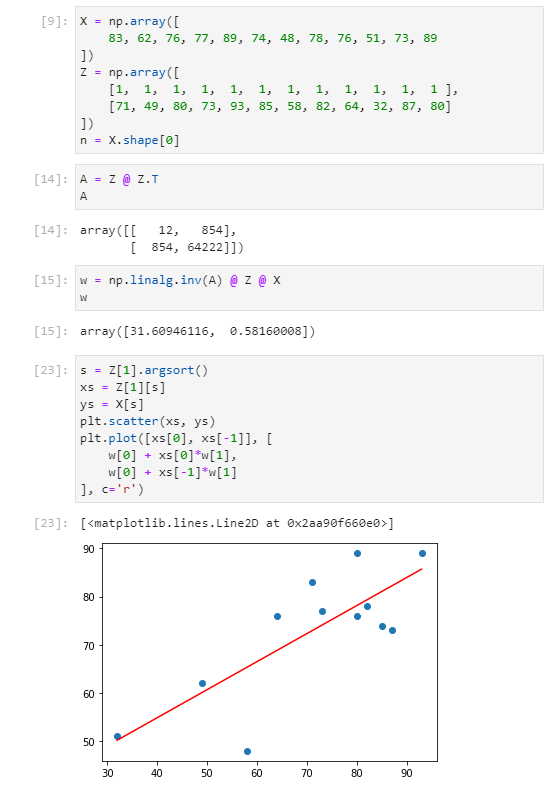
\includegraphics[width=0.8\textwidth]{task4.png}
\end{figure}
\pagebreak

Отримали рівняння регресії
$$\hat y = 31.6 + 0.58 x$$

\begin{mdframed}[style=ans]
    $$\beta_0 = 31.6;\quad \beta_1 = 0.58$$
    $$\hat y = 31.6 + 0.58 x$$
\end{mdframed}

Спрогнозуємо бал підсумкової контрольної студенту, що отримав 84 бали за модульну:
$$y' = 31.6 + 0.58 \cdot 84 = 80.46$$

\begin{mdframed}[style=ans]
    $$\hat y = 80.46$$
\end{mdframed}

Помітимо, що значення 84 всередині навчального діапазону, тобто маємо справу з інтерполяцією.
Шукаємо $0.95$-довірчий інтервал для прогнозованого значення інтерполяції.

$$t_0 = \frac{(\hat y_0 - y_0) \sqrt{n-2}}{\sqrt{\frac{1}{n}S(\hat \beta) + \frac{(\bar x - x_0)^2}{S_{xx}}}}$$
де $n$ - к-сть спостережень, $y_0$ - істинне значення значення, $\hat \beta$ - обчислена оцінка параметрів, \\ 
$S(\beta) = \left\|X - Z\beta\right\|^2$, \quad
$S_{xx} = \sum_{i=1}^n (x_i-\bar x)^2$.

$$S(\hat \beta) = 27.14$$
$$S_{xx} = 1902.0$$

Інтервал:
$$P(g_1 < t_0 < g_2) = 0.95$$
$$t_0 \sim t(n-2)$$
Центральний інтервал матиме такі межі: $$g_1 = t_{\frac{1-\gamma}{2};n-2}; g_2 = t_{\frac{1+\gamma}{2};n-2}$$

$$g_1 < \frac{(\hat y_0 - y_0) \sqrt{n-2}}{\sqrt{\frac{1}{n}S(\hat \beta) + \frac{(\bar x - x_0)^2}{S_{xx}}}} < g_2$$
$$\sqrt{\frac{1}{n}S(\hat \beta) + \frac{(\bar x - x_0)^2}{S_{xx}}} \cdot \frac{g_1}{\sqrt{n-2}} < \hat y_0 - y_0 < \sqrt{\frac{1}{n}S(\hat \beta) + \frac{(\bar x - x_0)^2}{S_{xx}}} \cdot \frac{g_2}{\sqrt{n-2}}$$
$$\hat y_0 - \sqrt{\frac{1}{n}S(\hat \beta) + \frac{(\bar x - x_0)^2}{S_{xx}}} \cdot \frac{g_2}{\sqrt{n-2}} < y_0 < \hat y_0 - \sqrt{\frac{1}{n}S(\hat \beta) + \frac{(\bar x - x_0)^2}{S_{xx}}} \cdot \frac{g_1}{\sqrt{n-2}}$$

Обчислюємо і отримуємо:
$$P(80.46 - 1.07 < y_0 < 80.46 + 1.07) = 0.95$$
\begin{mdframed}[style=ans]
    $$P(79.39 < y_0 < 81.53) = 0.95$$
\end{mdframed}

\noindent\rule{\textwidth}{0.4pt}

\section*{№5}
\subsection*{a)}

\begin{figure}[h]
    \centering
    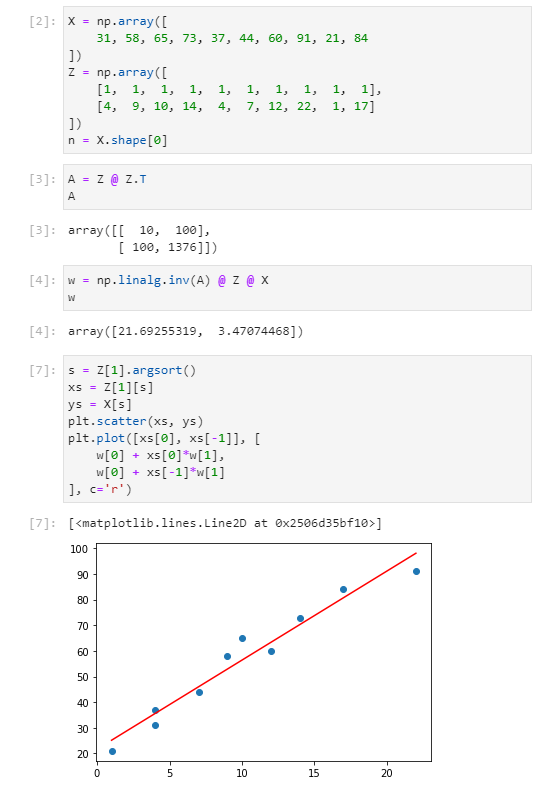
\includegraphics[width=0.7\textwidth]{task5.1.png}
\end{figure}
\pagebreak

Маємо рівняння прямої 
$$\hat y = 21.69 + 3.47 \cdot x$$

\subsection*{b)}
$$\hat y = 21.69 + 3.47 \cdot 10 = 56.4$$

"10 годин" - всередині навчального інтервалу. інтерполяція. Інтервал:
$$\hat y_0 - \sqrt{\frac{1}{n}S(\hat \beta) + \frac{(\bar x - x_0)^2}{S_{xx}}} \cdot \frac{g_2}{\sqrt{n-2}} < y_0 < \hat y_0 - \sqrt{\frac{1}{n}S(\hat \beta) + \frac{(\bar x - x_0)^2}{S_{xx}}} \cdot \frac{g_1}{\sqrt{n-2}}$$

Обчислюємо і маємо:
$$P(55.26 < y_0 < 57.54) = 0.95$$

\subsection*{c)}
Гіпотеза
$$y \sim \mathcal N (a+bx, \sigma^2)$$
$$H_0 : b=3$$
$$H_1 : b>3$$
$$\alpha = 0.01$$

Статистика критерію значущості окремого параметра має вигляд
$$t_0 = \frac{\hat b - b}{\sqrt{S(\hat a, \hat b) \cdot \left(A^{-1}\right)_{22}}}\sqrt{n-k} \sim t(n-k)$$
(Зауваження: $k=2$)

$$\hat a = 21.69; \quad \hat b = 3.47$$
$$S(\hat a, \hat b) = 14.94; \quad \left(A^{-1}\right)_{11} = 0.00266$$

Обчислюємо і маємо
$$|t_0| = 1.73 < t_{crit} = t_{1-\frac{0.01}{2};n-2} = 3.35$$

Отже, нульову гіпотезу \textbf{не} можна відхиляти. Можна зробити висновок, що в середньому кожна додаткова 
година пiдготовки до контрольної роботи пiдвищує бал на \textbf{менше} нiж три пункти.

Тобто, різниця $\hat b - b = 0.47$ недостатня для статистичної значимості результатів.

обчислення:
\begin{figure}[h]
    \centering
    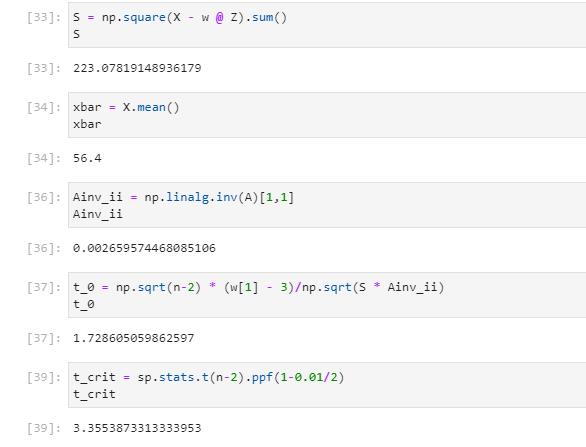
\includegraphics[width=0.7\textwidth]{task5.c.png}
\end{figure}

\subsection*{d)}
Будуємо 0.95-довірчий інтервал для $b$ в термінах попереднього пункту.

Маємо таку центральну статистику для b:
$$t_0 = \frac{\hat b - b}{\sqrt{S(\hat a, \hat b) \cdot \left(A^{-1}\right)_{11}}}\sqrt{n-k-1} \sim t(n-k-1)$$

$$P(g_1 < \frac{\hat b - b}{\sqrt{S(\hat a, \hat b) \cdot \left(A^{-1}\right)_{11}}}\sqrt{n-k-1} < g_2) = \gamma$$
$$\frac{\sqrt{S(\hat a, \hat b) \cdot \left(A^{-1}\right)_{11}}}{\sqrt{n-k-1}} g_1 < (\hat b - b) < \frac{\sqrt{S(\hat a, \hat b) \cdot \left(A^{-1}\right)_{11}}}{\sqrt{n-k-1}} g_2$$
$$\hat b - \frac{\sqrt{S(\hat a, \hat b) \cdot \left(A^{-1}\right)_{11}}}{\sqrt{n-k-1}} \cdot t_{\frac{1+\gamma}{2};n-2-1} < b < \hat b + \frac{\sqrt{S(\hat a, \hat b) \cdot \left(A^{-1}\right)_{11}}}{\sqrt{n-k-1}} \cdot t_{\frac{1+\gamma}{2};n-2-1}$$

Обчислюємо і маємо
$$P(2.84 < b < 4.1) = 0.95$$

\begin{figure}[h]
    \centering
    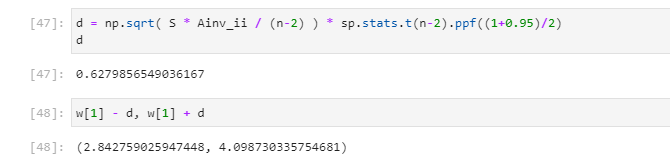
\includegraphics[width=0.7\textwidth]{task5.d.png}
\end{figure}

\pagebreak
\section*{№6}

$$y = ax^b$$
$$\ln y = \ln a + b \ln x$$
$$y' = a' + b' x'$$

Маємо модель лінійної регресії.
Обчислюємо та отримуємо

$$\hat a' = 8.777; \quad \hat b' = -1.04$$
$$\hat a = 6481; \quad \hat b = -1.04$$
$$\hat y = 6481 \cdot x ^ {-1.04}$$

\begin{figure}[h]
    \centering
    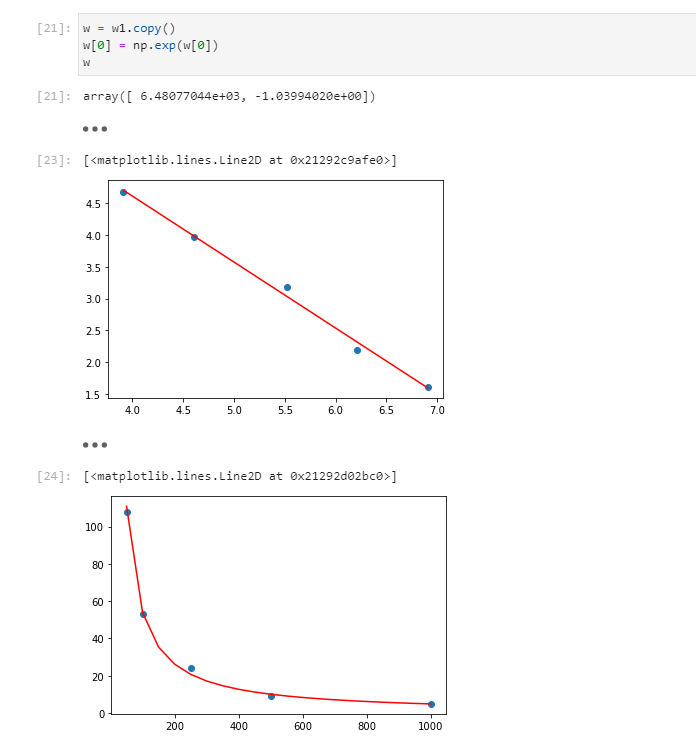
\includegraphics[width=0.7\textwidth]{task6.png}
\end{figure}

Оцінка вартості виробництва партії з 300 деталей:
$$y_{300} = 6481 \cdot 300 ^ {-1.04} = 17.2$$

\pagebreak

\section*{№7}

Будуємо регресію із $n=6, k=3$.

\begin{figure}[h]
    \centering
    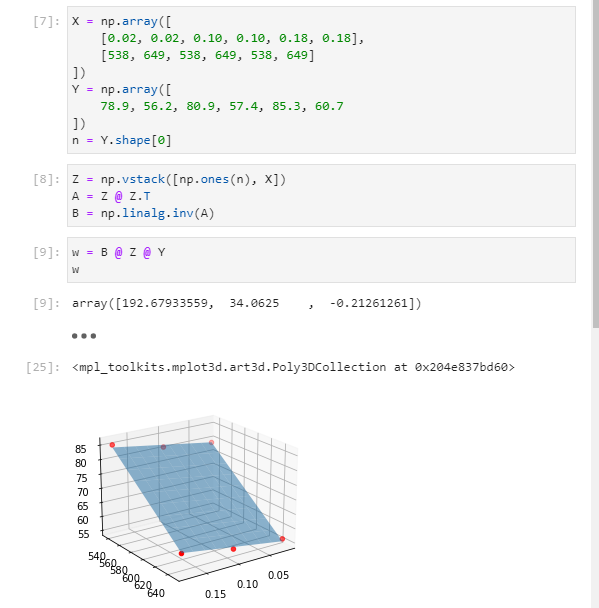
\includegraphics[width=0.8\textwidth]{task7.png}
\end{figure}

$$\hat y = 192.68 + 34.06 x_1 - 0.2126 x_2$$

$$\hat y_0 = 192.68 + 34.06 \cdot 0.14 - 0.2126 \cdot 593 = 71$$

\pagebreak

\section*{№8}
Доповнюємо Z стовпцями $(x_i^2)$ та обчислюємо регресію із $k=3$.

\begin{figure}[h]
    \centering
    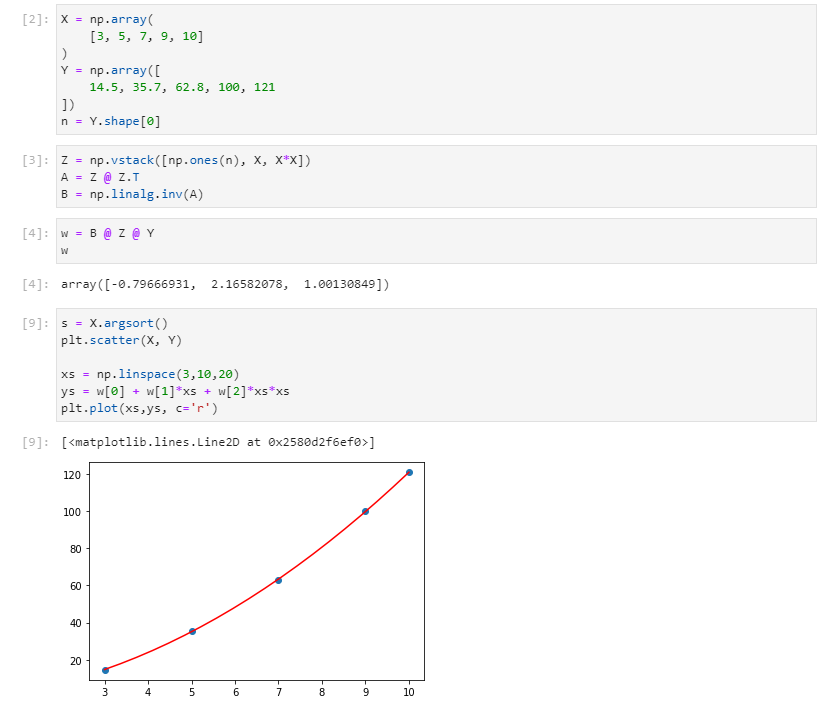
\includegraphics[width=0.8\textwidth]{task8.png}
\end{figure}

$$\hat y = -0.8 + 2.17 x + 1 \cdot x^2$$
Тобто прискорення $a = 1$.

Вже вивели такий вигляд довірчого інтервалу:
$$\hat a - \frac{\sqrt{S(\hat \beta) \cdot \left(A^{-1}\right)_{33}}}{\sqrt{n-k}} \cdot t_{\frac{1+\gamma}{2};n-3} < a < \hat a + \frac{\sqrt{S(\hat \beta) \cdot \left(A^{-1}\right)_{33}}}{\sqrt{n-k}} \cdot t_{\frac{1+\gamma}{2};n-3}$$

Обчислюємо і маємо
$$P(0.744 < a < 1.259) = 0.95$$

Також маємо наступну статистику для $\sigma^2$:
$$\frac{S(\hat \beta)}{\sigma^2} \sim \chi^2(n-k)$$

$$g_1 = \chi^2_{\frac{1-\gamma}{2};n-k}; \quad g_2 = \chi^2_{\frac{1+\gamma}{2};n-k}$$
$$P\left(g_1 < \frac{S(\hat \beta)}{\sigma^2} < g_2\right) = \gamma$$
$$P\left(\frac{S(\hat \beta)}{g_2} < \sigma^2 < \frac{S(\hat \beta)}{g_1}\right) = \gamma$$

Обчислюємо і маємо
$$P(0.12 < \sigma^2 < 17.4) = 0.95$$

Обчислення:
\begin{figure}[h]
    \centering
    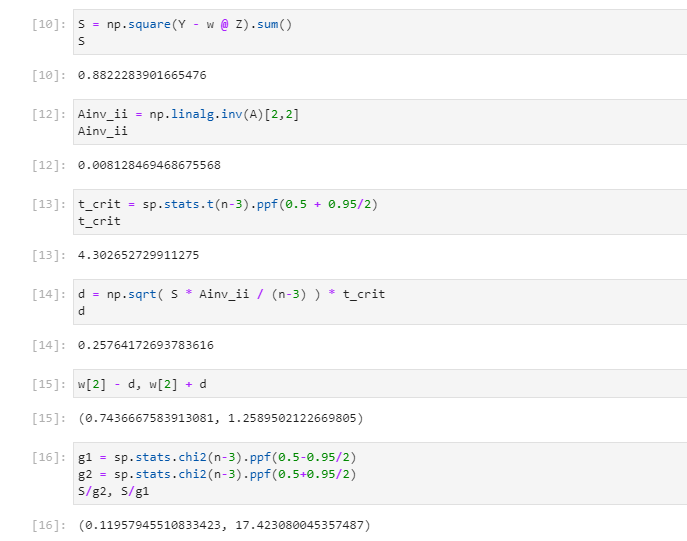
\includegraphics[width=0.8\textwidth]{task8.1.png}
\end{figure}


% \noindent\rule{\textwidth}{0.4pt}
\pagebreak

\section*{№9}
Доповнюємо Z стовпцями $(x_i^2)$ та обчислюємо регресію із $k=3$.

\begin{figure}[h]
    \centering
    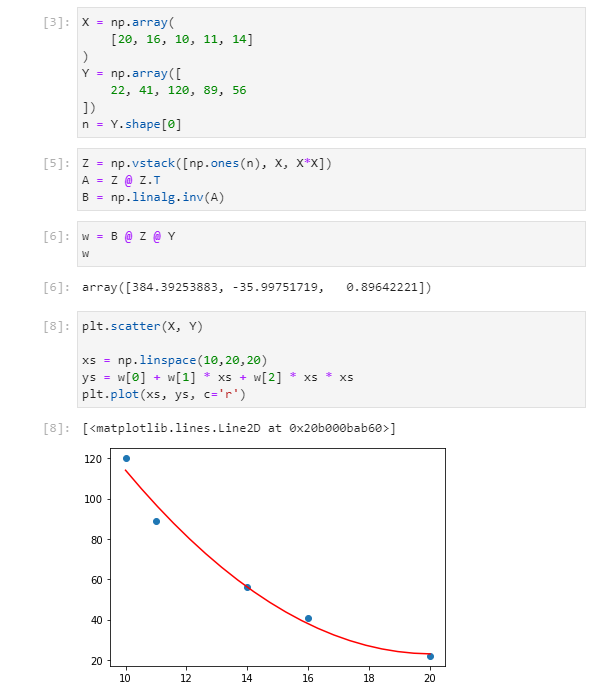
\includegraphics[width=0.8\textwidth]{task9.png}
\end{figure}

$$\hat y = 384.4 - 36 x + 0.895 x^2$$

Перевіримо гіпотезу ($\alpha=0.05$)
$$H_0 : \beta_2 = 0$$
$$H_1 : \beta_2 \ne 0$$

Запишемо вже знайому статистику
$$t_0 = \frac{\hat \beta_2 - 0}{\sqrt{S(\beta) \cdot \left(A^{-1}\right)_{33}}}\sqrt{n-k} \sim t(n-k); \quad t_{crit} = t_{1-\frac{\alpha}{2}; n-k}$$

Обчислюємо
$$t_0 = 2.94 < t_{crit} = 4.3$$

Отже, \textbf{не можна} відхилити нульову гіпотезу.
Залежність, скоріш за все, не має сенсу описувати параболічно.

Обчислення:
\begin{figure}[h]
    \centering
    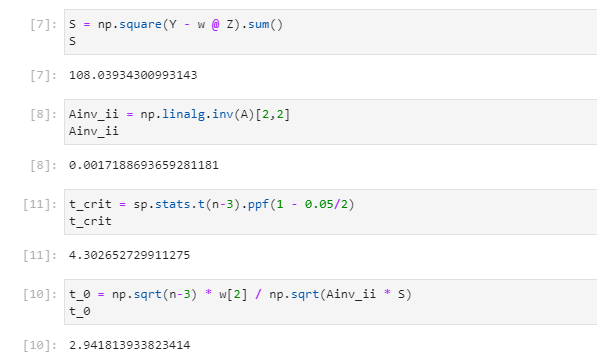
\includegraphics[width=0.8\textwidth]{task9.1.png}
\end{figure}

\noindent\rule{\textwidth}{0.4pt}

\section*{№10}
Оцінкою максимальної правдоподібності для коефіцієнта кореляції $\rho$ є
$$r = \frac{\sum_{i=1}^n y_i (x_i-\bar x)}{\sqrt{\sum_{i=1}^n(x_i-\bar x)^2 \sum_{i=1}^n (y_1-\bar y)^2}} = \frac{S_{xy}}{\sqrt{S_{xx}S_{yy}}}$$

Обчислюємо і отримуємо
$$r = 0.936$$

Значення близьке до 1, а значить регресія є значущою - є сенс вважати, що існує лінійна залежність.\\
А $r^2 = 0.876$ вказує на те, що лінійна модель пояснює 87\% варіативності.\\  

Статистикою критерію гіпотези $(H_0: \rho = 0)$ проти $(H_1 : \rho \ne 0)$  є
$$z = \frac{\sqrt{n-3}}{2}\ln \frac{1+r}{1-r}$$
$$z_{crit}: \quad |z| > u_{1-\frac{\alpha}{2}}$$

$$z = 4.5 > z_{crit} = 2.576$$

Отже, можна відхилити нульову гіпотезу про некорельованість цих наборів даних. \\
Тобто, можна прийняти, що дані корельовані між собою.

\end{document}

